\documentclass[11pt]{article}
\usepackage{graphicx}
\oddsidemargin -0.1in
\textwidth 6.5in
\topmargin -0.5in
\textheight 9in

\begin{document}
\pagestyle{empty}

\begin{Large}
\begin{center}
{\bf Revised Version of Homework 2}\\
CS626 Data Analysis and Simulation
\end{center}
\end{Large}
\begin{large}
\begin{center}
Name: Sidi Chang\\
%Out: Wednesday, 1/21\\
Due: 12:30 p.m., Tuesday, 5/31
\end{center}
\end{large}
\section{Question 1}
\subsection{The first trace: $wdev_0.csv$}
(a). [\textbf{inter arrival}] If I follow the equation from the slides shown $r_i=a_i-a_{i-1}$, I will start from the first number as 0 since 1.281664e+17 is too big. Then using R to do the calculation, we can find that: \\
\begin{table}[htdp]
\caption{metrics for $wdev_0$}
\begin{center}
\begin{tabular}{c|c|c|c}
\hline
Mean & Var & SD & C.V. \\
\hline
5290159 & 5.767035e+14 & 24014653 & 4.539496 \\
\hline
\end{tabular}
\end{center}
\label{metrics for $wdev_0$}
\end{table}%

The transient of the mean is below:  \\
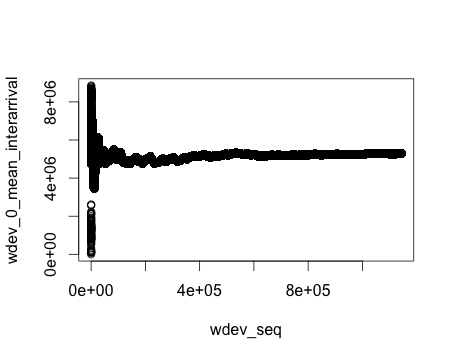
\includegraphics[scale=0.5]{transient_mean1.png}
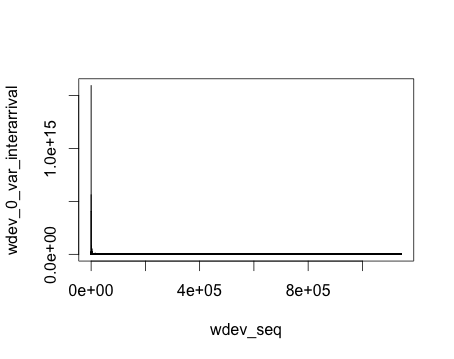
\includegraphics[scale=0.5]{SD_1.png} \\
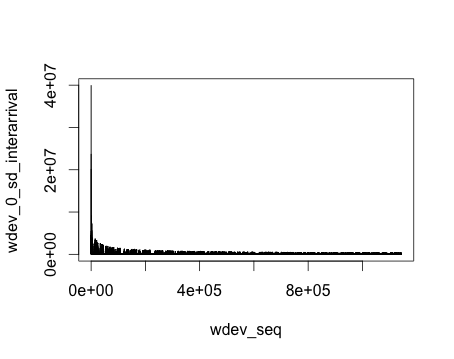
\includegraphics[scale=0.5]{SD11.png}
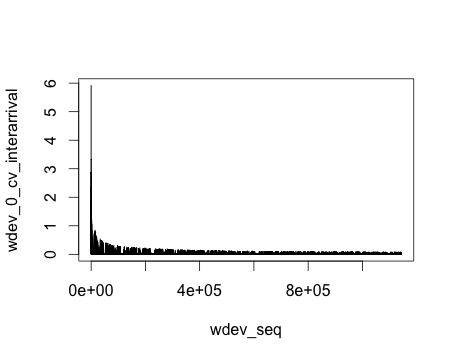
\includegraphics[scale=0.5]{CV1.png} \\
~~~[\textbf{service time}] 
\begin{center}
\begin{tabular}{c|c|c|c}
Mean & Var & SD & C.V. \\
\hline
3649.102 & 295778230 & 17198.2 & 4.712995 \\
\end{tabular}
\end{center}
The graph is as blow: \\
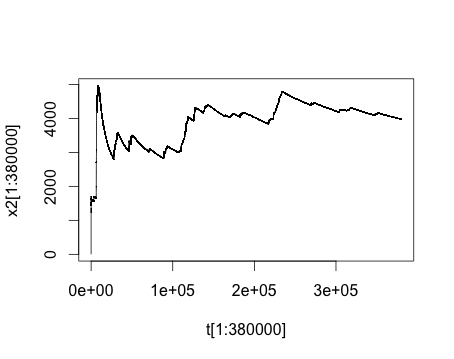
\includegraphics[scale=0.5]{mean2.png}
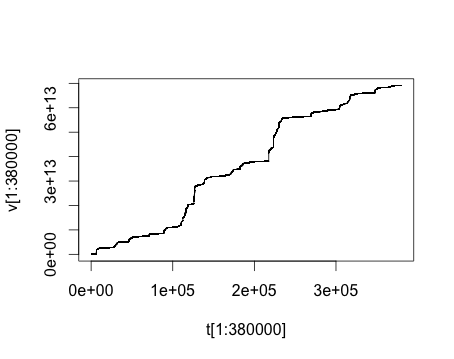
\includegraphics[scale=0.5]{v2.png}  \\
\includegraphics[scale=0.5]{SD2.png}
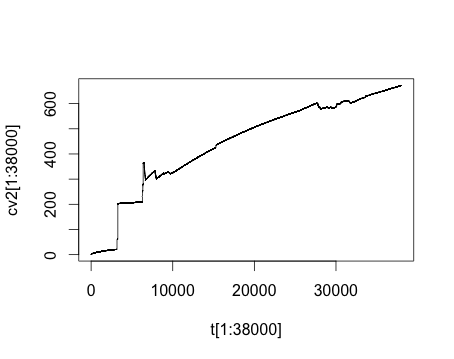
\includegraphics[scale=0.5]{CV2.png} 




(b). First, I draw the histograms of the whole graph and it is blow using bins 60: \\
\begin{center}
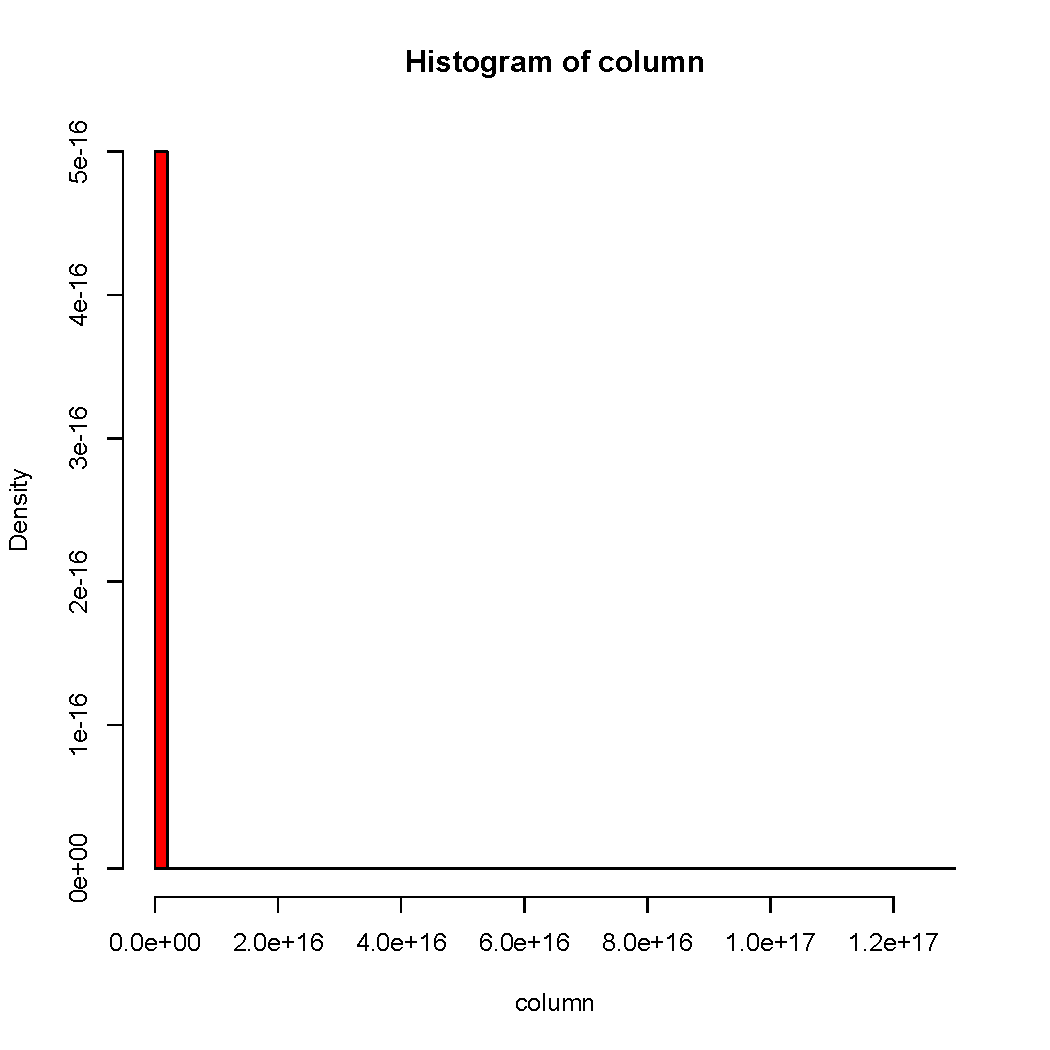
\includegraphics[scale=0.5]{trace1_1_full.pdf}
\end{center}
We can see the graph is so ugly and there is no meaning to draw pdf and cdf for this graph, then I find a solution, I get rid of the first big data and also just make the data restricted to (0,50000000) which contains $90\%$ of the numbers. Then I draw the graph with different bins: \\

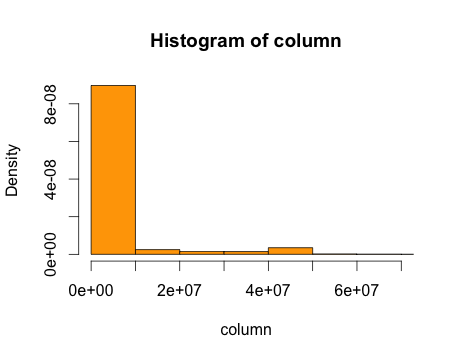
\includegraphics[scale=0.5]{Rplot_2.png}
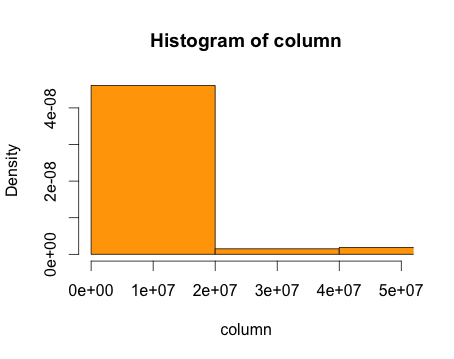
\includegraphics[scale=0.5]{Rplot_50000000.png} \\
The first bin is 60 and the second bin is 40, we can see 60 is better. Then I draw the pdf and cdf of inter-arrival: \\
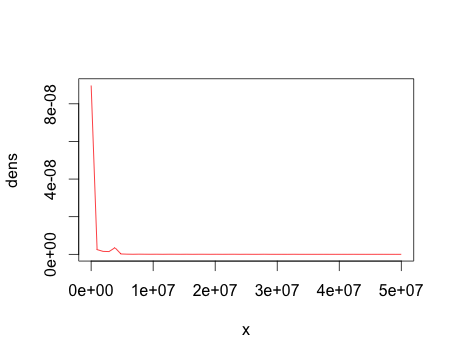
\includegraphics[scale=0.5]{1_pdf_inter_arrival.png}
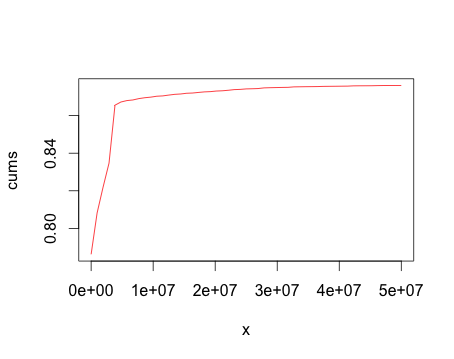
\includegraphics[scale=0.5]{1_cdf_inter_arrival.png} \\
Then I also do something for the service time, first I draw the graph for it to see what will happen: 
\begin{center}
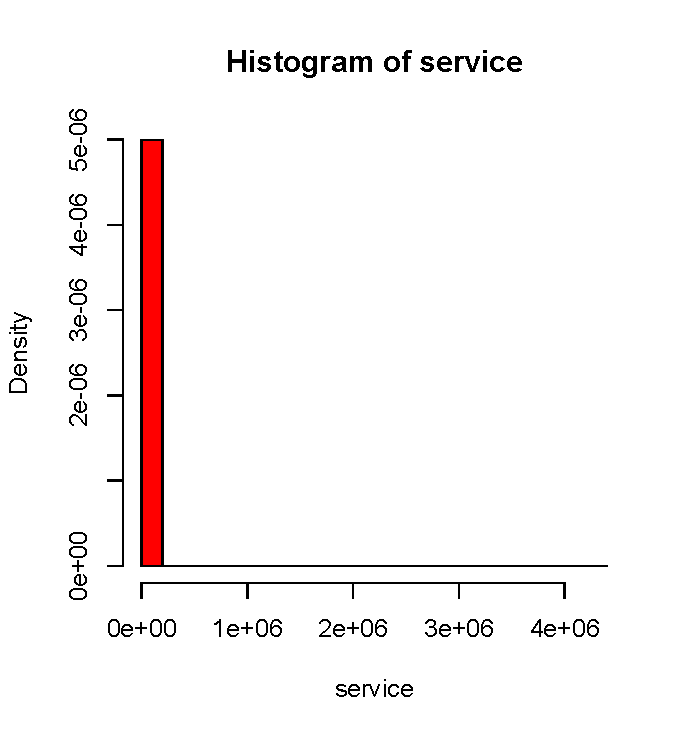
\includegraphics[scale=0.5]{trace1_service1.pdf}
\end{center}
Also we can see the graph is terrible like this. So I also do some cut and only take (0,100000) and bins=330, we can get histogram below: \\
\begin{center}
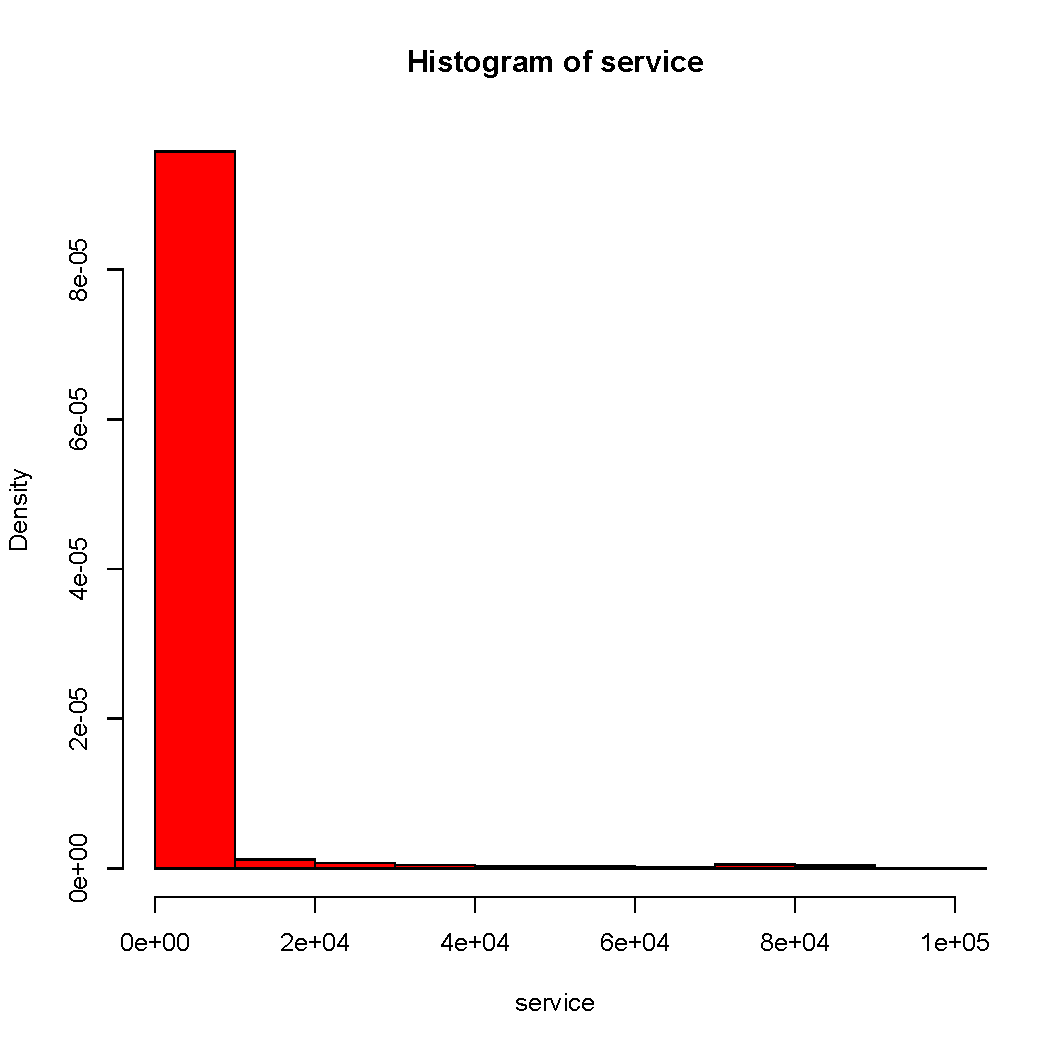
\includegraphics[scale=0.36]{trace1_service2.pdf}
\end{center}
Then we can get the pdf and cdf of the service time: \\
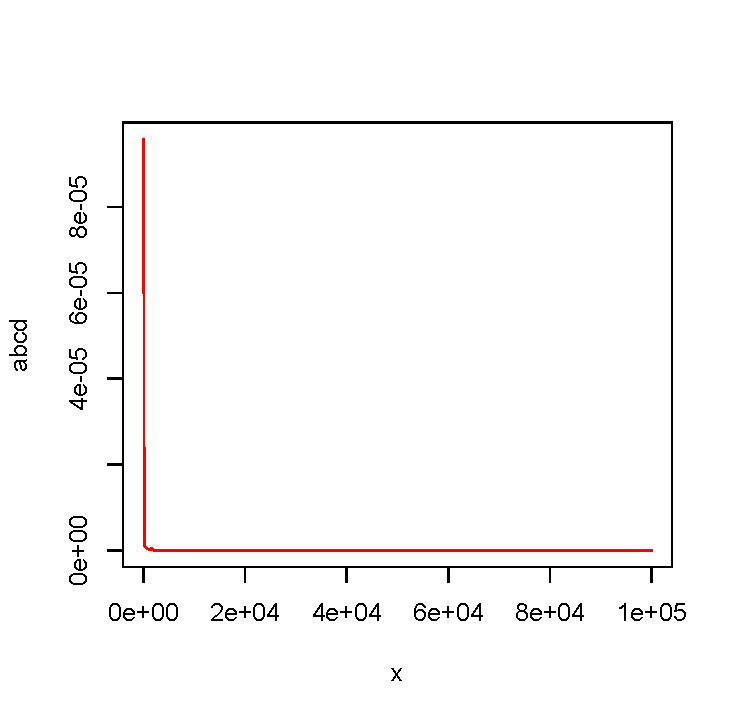
\includegraphics[scale=0.5]{trace1_2_pdf.pdf}
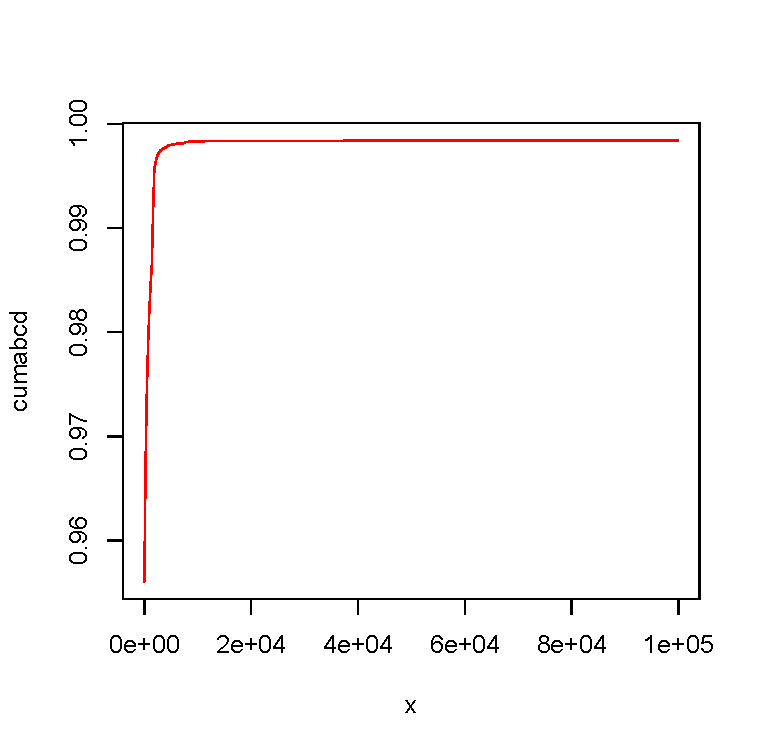
\includegraphics[scale=0.5]{trace1_2_cdf.pdf} \\
~~~[\textbf{Autocorrection function}]~There is a function in R called acf: \\
\includegraphics[scale=0.5]{acf1.png}
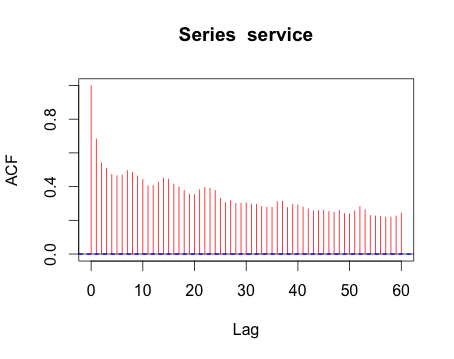
\includegraphics[scale=0.5]{acf2.png}


\subsection{\textbf{Trace 2: $Proj_3$}}
~~~(a) First the mean, var, SD and C.V. As I learned from the first trace, I decided to start with arrival[1], which means when the first arrival comes, I start to record the time. \\
Inter-arrival Time: Mean is 3664617, Var is 5.9327e+17, SD is 770240222, C.V. is 210.18. Then the transient measure:  \\
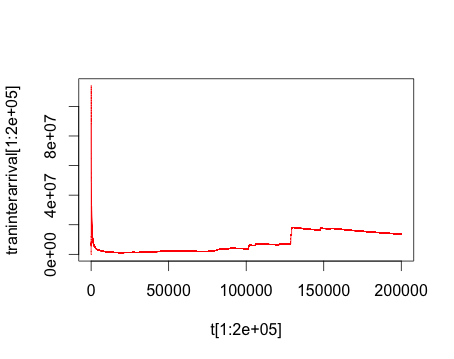
\includegraphics[scale=0.5]{traninterarrival2.png}
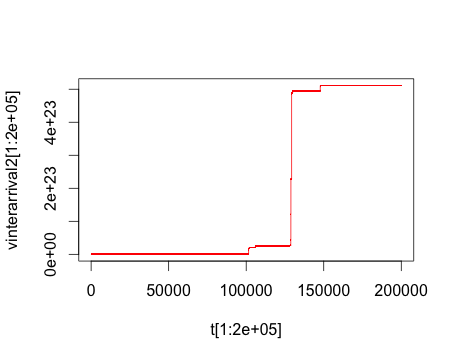
\includegraphics[scale=0.5]{vinterarrival2.png} \\
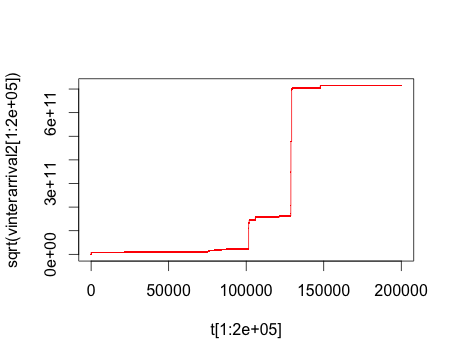
\includegraphics[scale=0.5]{SDinterarrival2.png}
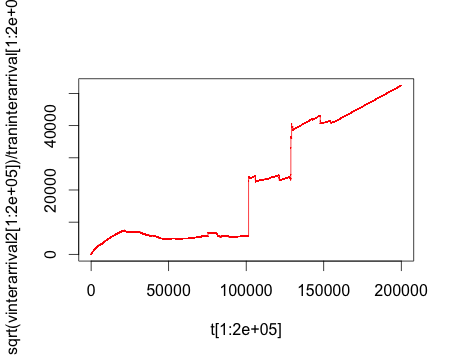
\includegraphics[scale=0.5]{CVinterarrival2.png} \\
Service time: Mean is 13247, Var is 572198941, SD is 23921, C.V. is 1.8058. The transient measure is as below: \\
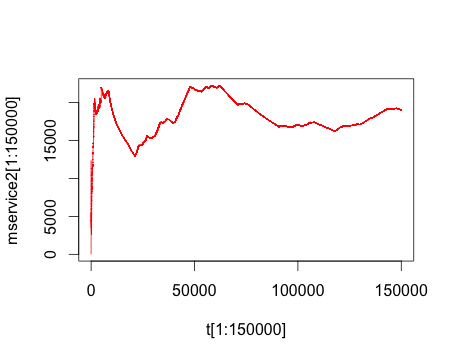
\includegraphics[scale=0.5]{mservice2.png}
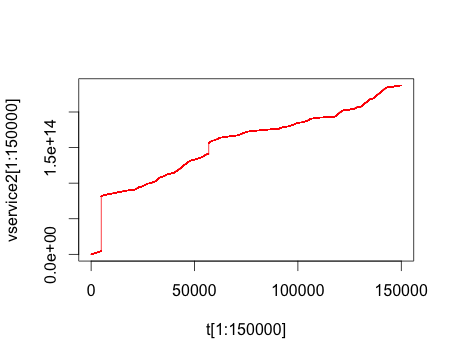
\includegraphics[scale=0.5]{vservice2.png} \\
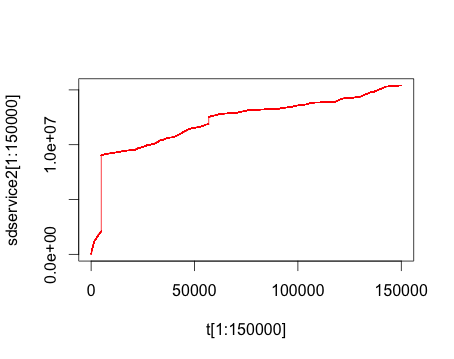
\includegraphics[scale=0.5]{SDservice2.png}
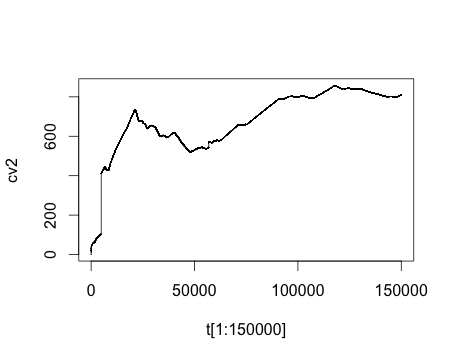
\includegraphics[scale=0.5]{CVservice2.png} \\
~~~(b) It is as shown below: (Above inter-arrival, below service)\\
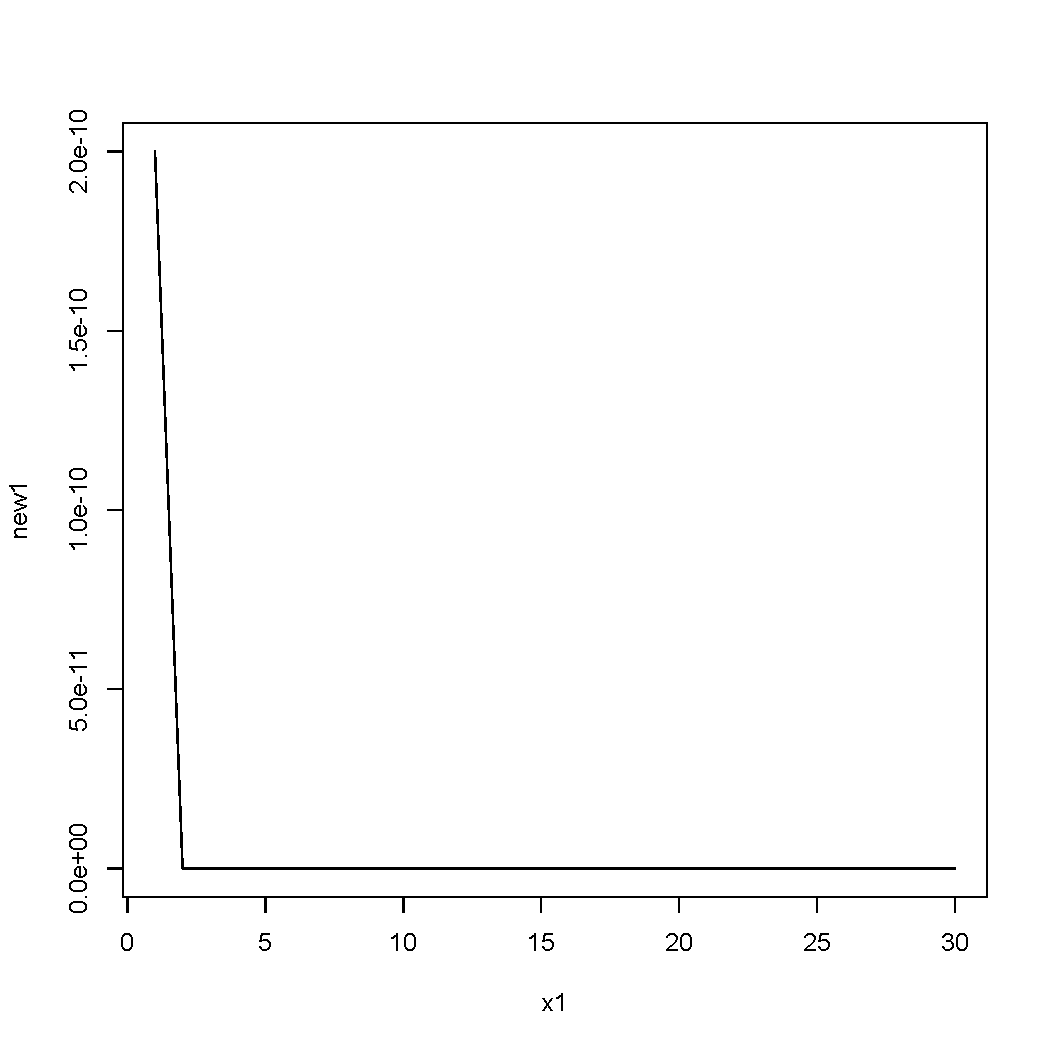
\includegraphics[scale=0.5]{pdfservice2.pdf}
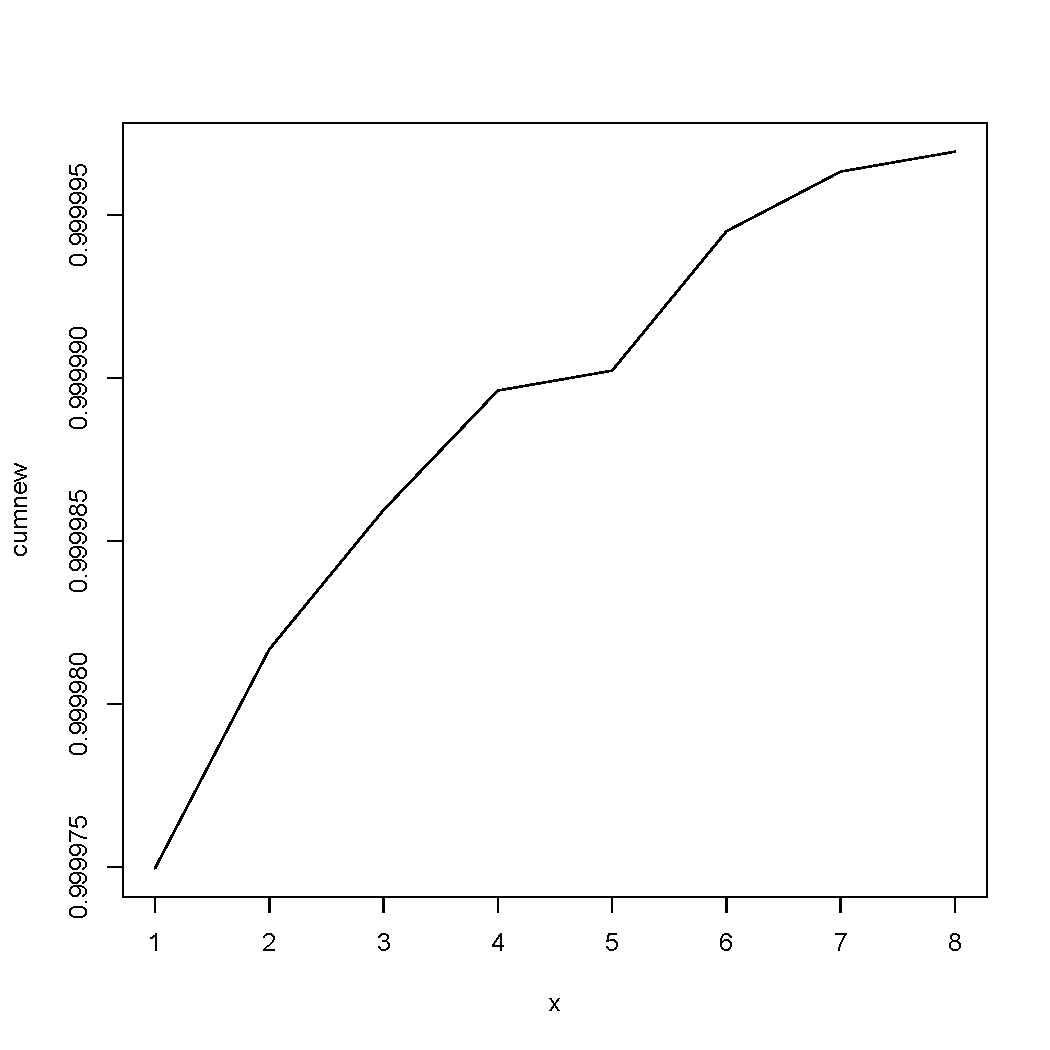
\includegraphics[scale=0.5]{cdfservice2.pdf}
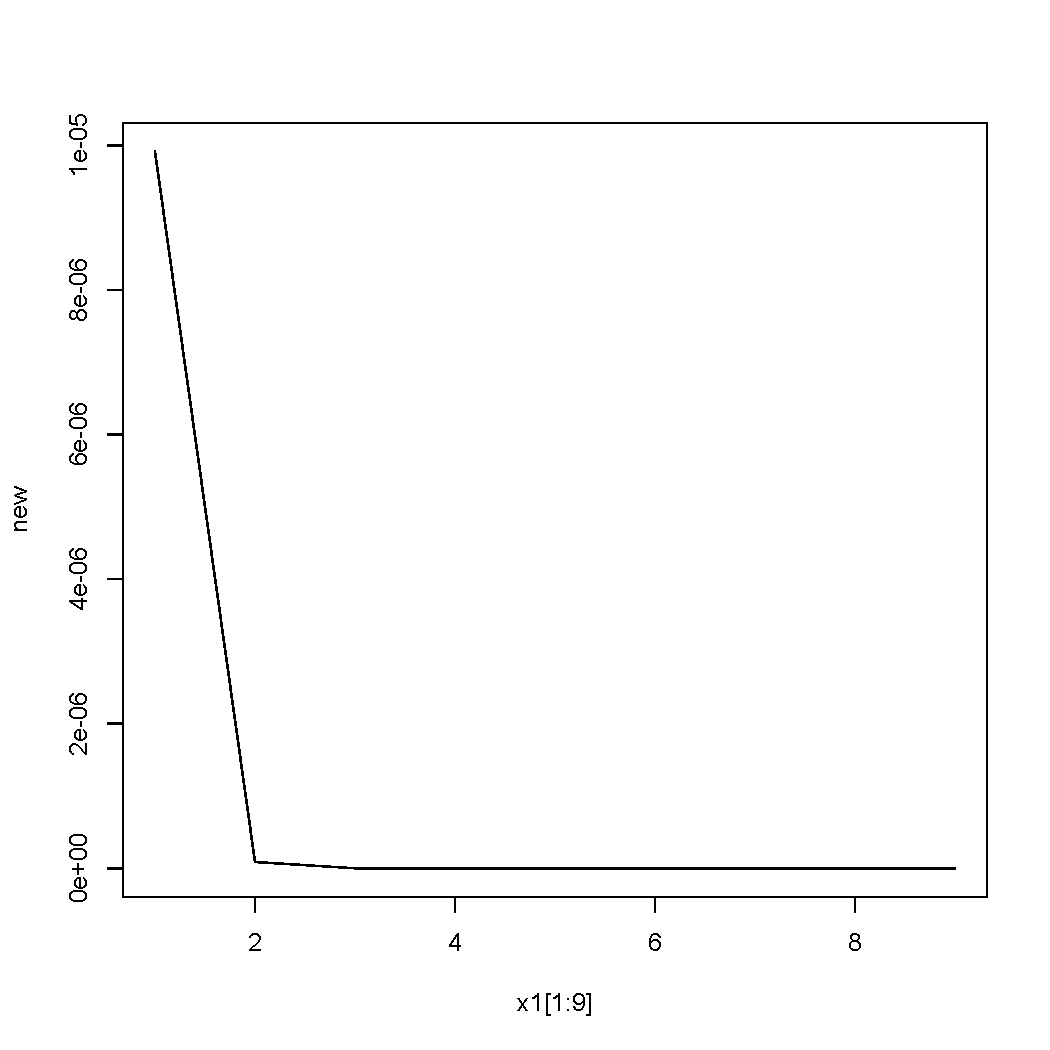
\includegraphics[scale=0.5]{pdf2222.pdf}
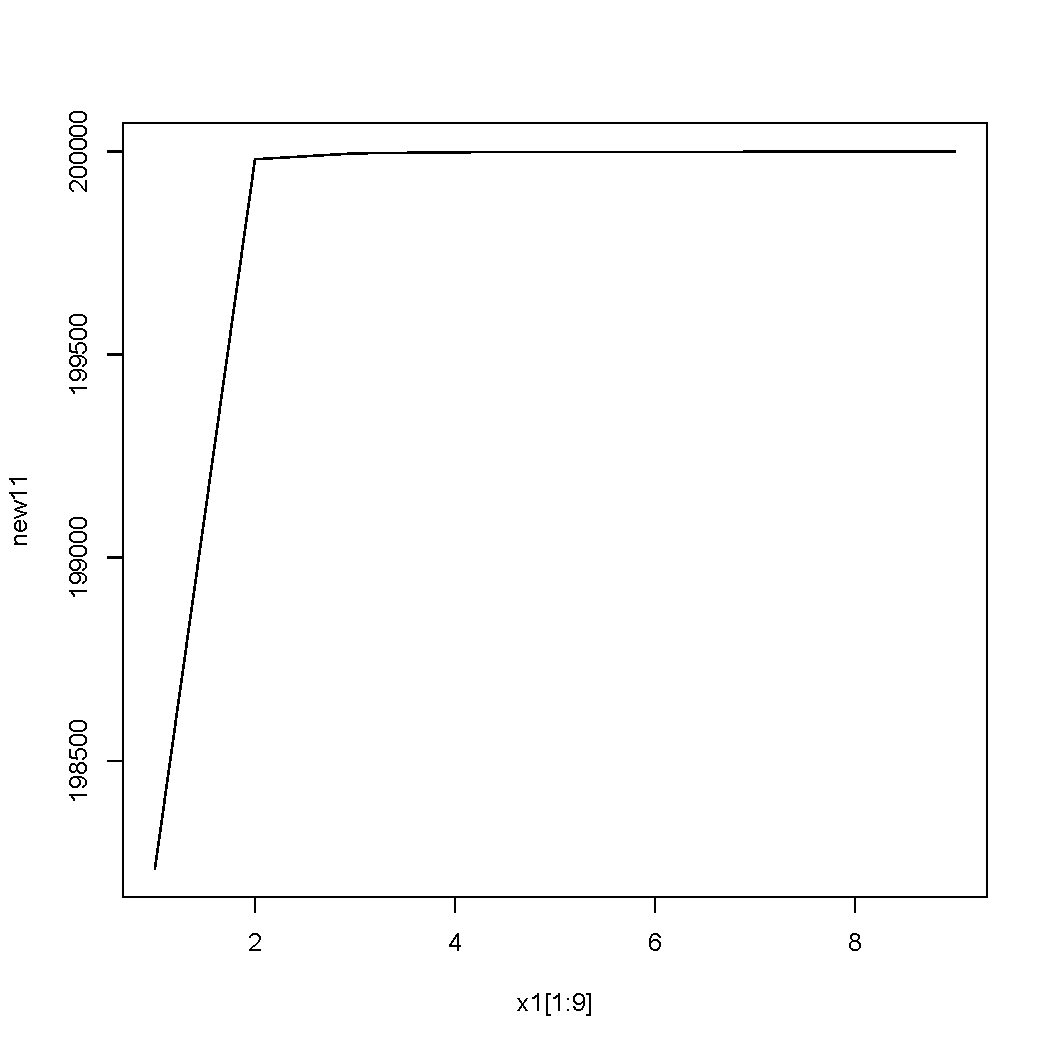
\includegraphics[scale=0.5]{cdf2222.pdf} \\
~~~(c) As below: \\
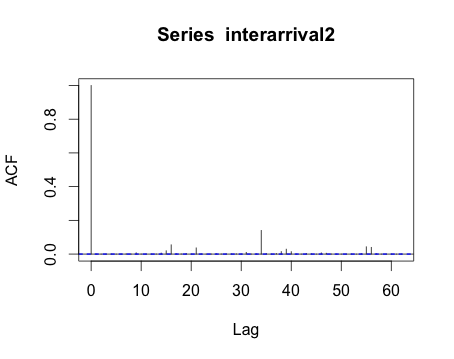
\includegraphics[scale=0.5]{acf22inter.png}
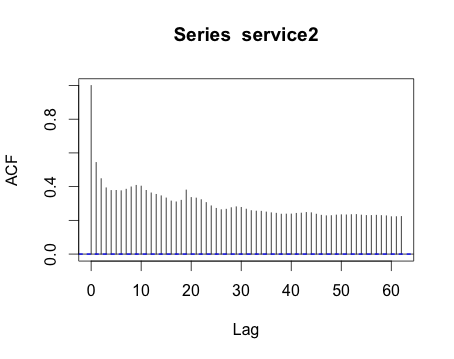
\includegraphics[scale=0.5]{acf22service.png}


\section{Question 2}
\subsection{Several metrics}
Firstly, I have to make the program starts at 0 cause the first number is too big, then retrieve the first 50,000 data sets out to do this question( Increase the efficiency of computing). I use the program ssq1.c and acs.c to get the result.
\begin{table}[htdp]
\caption{metrics for $wdev_0$}
\begin{center}
\begin{tabular}{c|c|c}
Mean delay time & system utilization & Average waiting queue length \\
\hline
69209.26 & 0.0058 & 0.002424
\end{tabular}
\end{center}
\label{default}
\end{table}%

\begin{center}
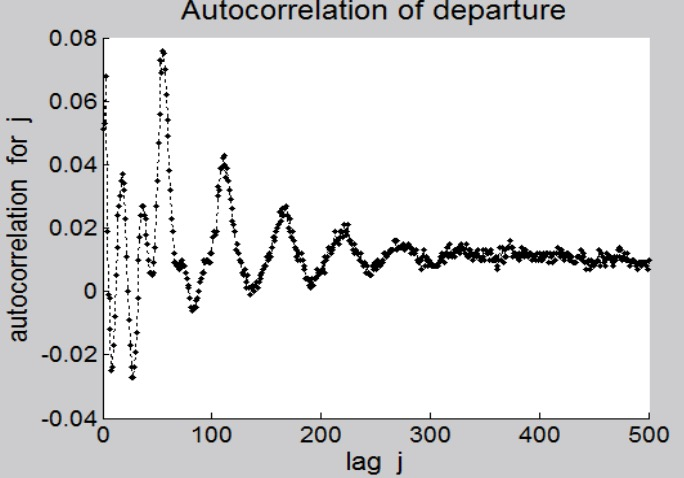
\includegraphics[scale=0.3]{C2_2000.png}
\end{center} 
~~(b)~I found a code on the website from Richmond University, he made the C code into R. Running his R program, I got the data below: \\
\begin{table}[htdp]
\caption{metrics for $wdev_0$ with exponential}
\begin{center}
\begin{tabular}{c|c|c}
Mean delay time & system utilization & Average waiting queue length \\
\hline
76491.77 & 0.0058 & 0.0032
\end{tabular}
\end{center}
\label{default}
\end{table}%
The original service time is as below, I just use the data from 1:380000 and got the graph: \\
\begin{center}
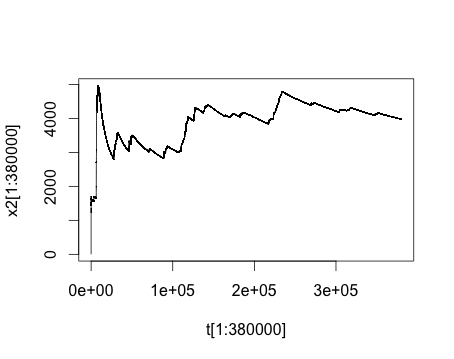
\includegraphics[scale=0.5]{mean2.png}
\end{center}
(c) I will choose the data from 100 to 100000, I will firstly show the data with trace data, then show the graph with exponential service times in the last question. So the graph is below: 
\begin{center}
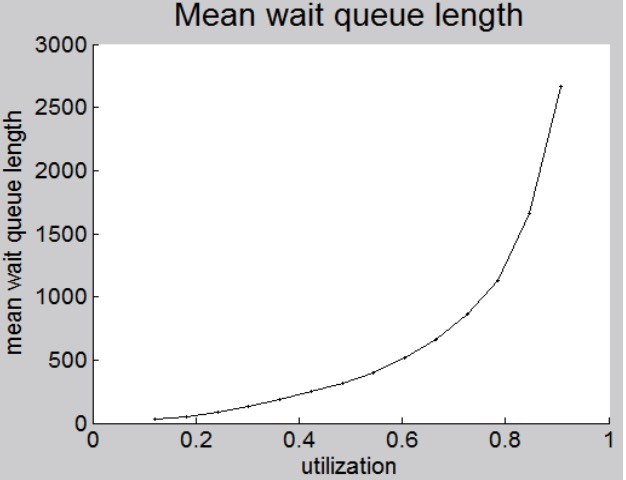
\includegraphics[scale=0.3]{wdev_0_meanwait_common.png}
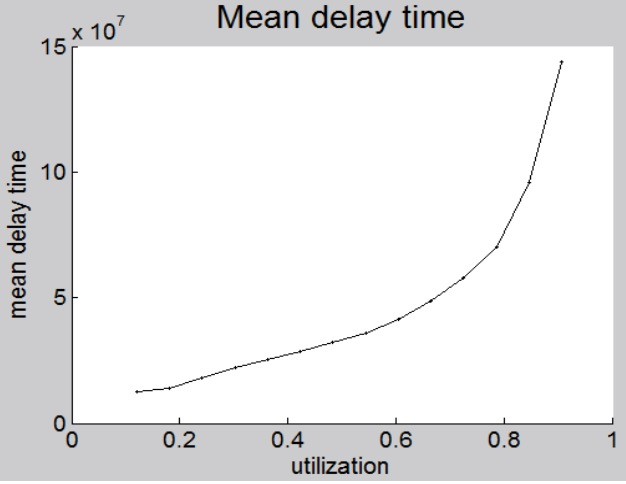
\includegraphics[scale=0.3]{wdev_0_mean_exponential.png}
\end{center}
Then in R, with the command hold on, we can plot several lines in one graph together, then I plot the line for utility 0.1-0.9 which is shown below: \\
\begin{center}
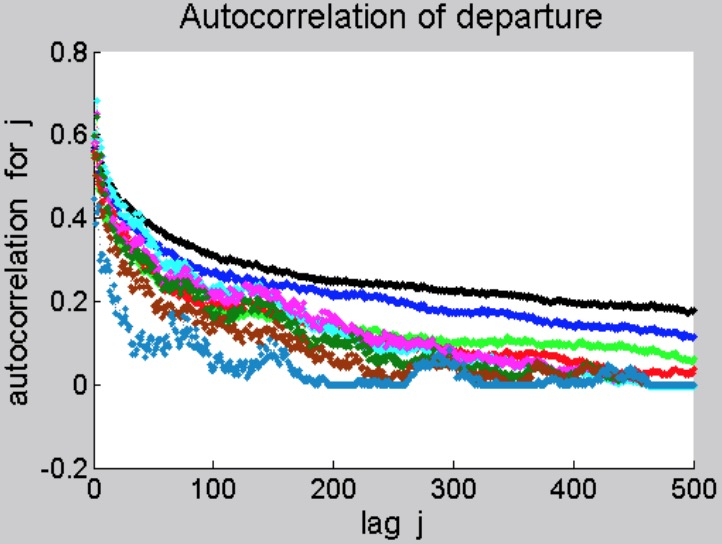
\includegraphics[scale=0.3]{hw2_auto}
\end{center}
Comment: 
\begin{enumerate}
\item
I found that using exponential service time, we can find that the system utility in the beginning has higher system usage, then it just goes down and in the end to a stable value. (This is the end of the first trace) 
\item
Using exponential service time and arrival time, obviously the delay time is smaller than the original track.
\item
From the autocorrelation of departure figure, we can find out that when j becomes larger, the autocorrelation becomes smaller but always bigger than 0.
\end{enumerate}


\end{document}
